\section{Reconfigurable Hardware}
A significant portion of the project's work involves exploiting reconfigurable hardware to vastly reduce the inference time of state-of-the-art neural networks. This section explains in more detail the technology and characteristics of the Field-Programmable Gate Arrays (FPGA).

\subsection{Landscape of Hardware for Computing}
The modern landscape of digital integrated circuits (IC) is very rich can be divided into numerous categories depending on the technology used and expected functionality \cite{14-najafi2017hardware}. A list of platform types is described below, with the emphasis of their suitability for neural networks applications.

\begin{itemize}
  \item \textbf{Central Processing Units (CPU)} - the most commonly found ICs that are at the core of personal computers, laptops and handheld devices. They are capable of executing a broad range of predefined instructions. As CPUs have become widely adopted in research long before the emergence of the other technologies from this list, they were the first platforms for the training and inference of neural networks with promising results back in the 1980s and 1990s for applications like high energy physics \cite{17-dagli1989applications} or biology \cite{16-wu1995neural}. Although possible to achieve speed-ups of over 10x the baseline performance with careful optimizations \cite{nn_cpu_optim}, CPUs are now consistently outperformed by more suitable technologies.

  \item \textbf{Graphic Processors (GPU)} - ICs specialized in graphics processing intended for displaying images. Since their original use case, due to the type of calculations involving matrix and vector operations, other applications related to cryptography and neural networks have also adopted GPUs as their main resource. In the former domain, cryptocurrency mining has transitioned from CPU to GPU to increase profitability \cite{19-iyer2018gpu}, while for the latter, the more powerful hardware drastically reduced training and inference times, thus allowing for deeper and more complex architectures yielding higher accuracy \cite{20-chen2020gpu-accelerated, 21-zhang2019recent}.

  \item \textbf{Application Specific Integrated Circuits (ASIC)} - as suggested by the name, those are the custom designed ICs heavily specialized for a particular use. It is hard to generalize them, as the use cases can cover any modern computing problem, but the commonality is a vast improvement in performance and power usage compared to more general purpose solutions. However, the long and expensive development process pose an extremely high barrier to entry for most users. Fortunately, off-the-shelf products like the Graphcore Intelligence Processing Units \cite{22-graphcoregraphcore} that are designed specifically with machine learning applications in mind as well as other custom designs \cite{23-knag2015sparse, 24-ramanaiah2011asic} are starting to offer a compelling platform for working with neural networks.

  \item \textbf{Field-Programmable Gate Arrays (FPGA)} - differently from the previous listed IC types, FPGAs are not manufactured for a specific use case, and in fact, they can be reprogrammed to be a platform for a different application at any time. The reprogrammability comes at a cost of performance and power consumption compared to ASICs \cite{25-boutros2018improve}, but at the same time outperforms GPUs in these regards \cite{27-nurvitadhi2017fpgas, 28-li2018gpu-outperforming}. It is also suggested, that with some technological improvements focused on ML applications, FPGAs can narrow the gap between ASICs without needing to stick to one particular design \cite{25-boutros2018improve, 26-nurvitadhi2016accelerating, 15-nurvitadhi2016accelerating}.

\end{itemize}

FPGAs offer an interesting trade-off between implementation effort and acceleration potential when it comes to neural networks and for that reason they have been chosen the target technology in this report. The following subsections give a closer look at some of their characteristics.

\subsection{High-Level Synthesis}
For many years, FPGAs have been modelled using register-transfer level (RTL) design abstraction with the use of hardware description languages like Verilog or VHDL. However, to increase productivity and allow for a more convenient design state space exploration, a more abstract modelling process called High-Level Synthesis (HLS) can be adopted. The design can be expressed in a software programming language like C or C++, which are automatically optimized and transformed to an equivalent RTL. This is especially beneficial in research, where compared to industrial environment, it is more likely that designers can afford slightly lower quality of results for increased productivity. In fact, a recent study shows that on average, only one third of design time and half of the lines of code are needed for an equivalent project done in HLS in comparison to RTL while the quality of results varies and can even outperform the RTL implementations \cite{30-lahti2019yet?}.

This report's work is based on Xilinx Vivado HLS design suite. When developing a solution, it is important to note, that the synthesis process can take a significant amount of time (a couple of hours on a modern powerful computer), and so there exist two simulation methods - a C-simulation that can quickly and directly evaluate a C/C++ benchmark against the software implementation of the design, and a more truthful, cosimulation that firstly synthesizes the design and the test bench to RTL and then performs an RTL simulation. A final, definitive evaluation of the results requires programming a target FPGA with the generated bit stream of the design and exchanging input/output data with a program that usually runs on a CPU.


\subsection{Latency, throughput, and hardware resource utilization}\label{latency-throughput-resources}
To understand the differences between hardware designs targeted at similar functionality, it is worth considering the following characteristics:

\begin{itemize}
  \item \textbf{Latency} - A time measure of a system between receiving an input signal and producing a \textit{corresponding} output. It is crucial in real-time processing where it has to be lower than the period between subsequent input samples. Depending on the application, latency in the microseconds range can be expected from an FPGA.
  \item \textbf{Throughput} - A rate of samples processed in a unit of time. For architectures that only start to process new elements after the previous one has finished, it is equal to latency. However, in modern ICs, especially in FPGAs, it is one of the defining metrics of performance and designs tend to exploit pipelining and parallelizability to marginally trade off their latency to increase it.
  \item \textbf{Resource utilization} - A more complicated, often multidimensional, metric that describes the raw number or ratio of total usage of the hardware components on an FPGA. Typically, the higher it becomes, the more power is drawn by an FPGA, however, it is most often used to guide the design process to avoid running out of a certain resource and potentially deploy an alternative method that can be implemented using a different, less contested resource.
\end{itemize}

To fully understand the trade-offs between designs, one cannot forget about the metric related to the specific task that is accelerated in hardware. In the case of this report, classification accuracy and AUC described in \autoref{ml-accuracy-auc-confusion}, will also play key roles in evaluating various configurations.


\subsection{Serial, parallel, and pipelined architectures}\label{serial-parallel-pipelined}
Hardware architectures use components that can be configured in different ways depending on the overall goal or a limiting factor. The high-level configurations  are displayed in figure \ref{fig:serial-parallel-pipelined} and can be described as follows:

\begin{itemize}
  \item \textbf{Serial} - elements are arranged in a chain, processing one after another. This way uses less resources than an equivalent parallel configuration.
  \item \textbf{Parallel} - elements share a common input and start processing data at the same time. This way ends in a lower latency than an equivalent serial configuration.
  \item \textbf{Pipelined} - a more sophisticated arrangement, in which subsequent processing blocks (that can be either placed serially or in parallel) form a pipeline of processing stations separated by simple storage elements called pipeline registers. This maximizes the usage of the design blocks, hence increasing throughput with a minimal sacrifice of latency and resource usage.
\end{itemize}

\begin{figure}[hpt!]
  \centering
  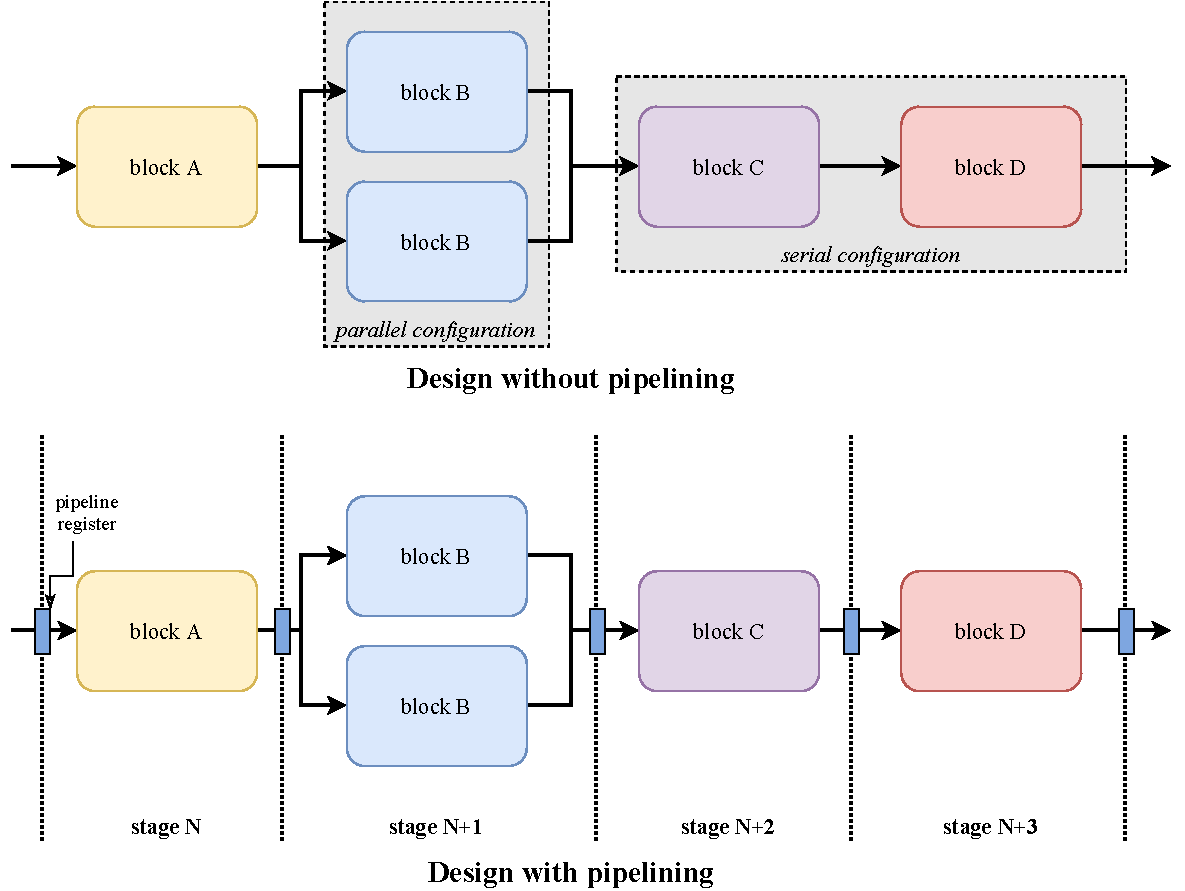
\includegraphics[trim={0cm 0cm 0cm 0cm}, width=0.75\textwidth, center]{background/serial_parallel_pipelined.pdf}
  \caption{Diagram comparing serial and parallel configurations as well as showcasing designs with and without pipelining}
  \label{fig:serial-parallel-pipelined}
\end{figure}

\pagebreak
\subsection{Pareto front and Roofline model}
To make an informed design decision, various architectures can be compared by arranging them on a dependency graph (e.g. latency vs resource usage) and observing the Pareto front - the set of solutions for which there are no better ones in regard to one quality given that the other measure is not worse. The slightly complex definition can be easily understood from figure \ref{fig:pareto}, which also highlights another use of this method - finding design configurations that are yet to be explored.

\begin{figure}[hpt!]
  \centering
  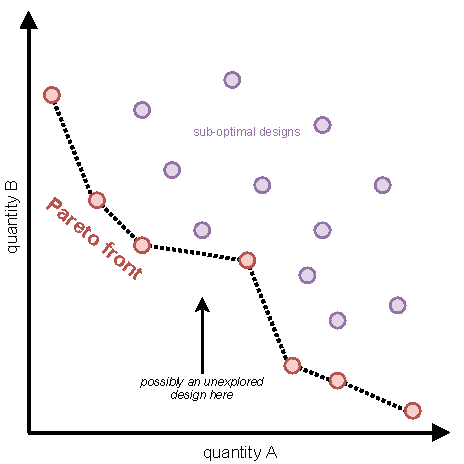
\includegraphics[trim={0cm 0cm 0cm 0cm}, width=0.5\textwidth, center]{background/pareto.pdf}
  \caption{Example graph with designs plotted against quantities A/B, Pareto front highlighted}
  \label{fig:pareto}
\end{figure}

\pagebreak
Another intuitive performance visualization comes in the form of the Roofline model, which compares the obtained results with theoretical limits coming from inherent hardware limitations like clock frequency or memory bandwidth. An example can be seen in fig \ref{fig:roofline}.

\begin{figure}[hpt!]
  \centering
  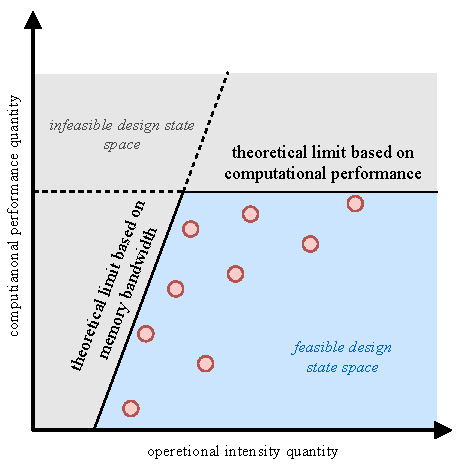
\includegraphics[trim={0cm 0cm 0cm 0cm}, width=0.5\textwidth, center]{background/roofline.pdf}
  \caption{Example graph with computational and memory bandwidth limitations showcasing the Roofline model}
  \label{fig:roofline}
\end{figure}


\maybe{some graphics to potentially add: fpga lattice, hls to rtl flow, rtl to bit stream flow}
\maybe{difficulty: rtl > hls > python hl4ml, draw comparison with assembly}
\maybe{FPGA are very hard-coded -> make the code deployable on any platform with optimal settings automatically}
\maybe{HLS is difficult, so coding hardware in Python is desired -> make it easy for engineers and physicists to design systems}
\maybe{Metaprogramming allows for optimizations and customisability}